%%%%%%%%%%%%%%%%%%%%%%%%%%%%%%%%%%%%%%%%%
% FRI Data Science_report LaTeX Template
% Version 1.0 (28/1/2020)
% 
% Jure Demšar (jure.demsar@fri.uni-lj.si)
%
% Based on MicromouseSymp article template by:
% Mathias Legrand (legrand.mathias@gmail.com) 
% With extensive modifications by:
% Antonio Valente (antonio.luis.valente@gmail.com)
%
% License:
% CC BY-NC-SA 3.0 (http://creativecommons.org/licenses/by-nc-sa/3.0/)
%
%%%%%%%%%%%%%%%%%%%%%%%%%%%%%%%%%%%%%%%%%


%----------------------------------------------------------------------------------------
%	PACKAGES AND OTHER DOCUMENT CONFIGURATIONS
%----------------------------------------------------------------------------------------
\documentclass[fleqn,moreauthors,10pt]{ds_report}
\usepackage[english]{babel}
\usepackage{tcolorbox} % add this to your preamble

\graphicspath{{fig/}}




%----------------------------------------------------------------------------------------
%	ARTICLE INFORMATION
%----------------------------------------------------------------------------------------

% Header
\JournalInfo{FRI Natural language processing course 2025}

% Interim or final report
\Archive{Project report} 
%\Archive{Final report} 

% Article title
\PaperTitle{Conversational Agent with Retrieval-Augmented Generation} 

% Authors (student competitors) and their info
\Authors{Blaž Grilj, Ana Poklukar, Kristjan Sever}

% Advisors
\affiliation{\textit{Advisors: Aleš Žagar}}

% Keywords
\Keywords{NLP, LLM, RAG}
\newcommand{\keywordname}{Keywords}


%----------------------------------------------------------------------------------------
%	ABSTRACT
%----------------------------------------------------------------------------------------

\Abstract{
Conversational agents based on large language models (LLMs) often struggle to provide accurate and up-to-date information due to their reliance on static pretrained knowledge. To address this, this project designs and implements a Retrieval-Augmented Generation (RAG) system that integrates live retrieval from Wikipedia to ground responses in current, factual data. Our approach combines semantic search with state-of-the-art LLMs in a modular pipeline, enabling dynamic access to relevant documents during answer generation. Through extensive experiments, we demonstrate that retrieval significantly improves correctness, relevance, and semantic alignment compared to non-augmented baselines. We also analyze the effects of retrieval parameters and language model choice, revealing that moderate retrieval sizes and well-tuned smaller models outperform larger models lacking retrieval synergy. Our work highlights the practical advantages and challenges of live retrieval augmentation in building reliable, context-aware conversational agents.
}

%----------------------------------------------------------------------------------------

\begin{document}

% Makes all text pages the same height
\flushbottom 

% Print the title and abstract box
\maketitle 

% Removes page numbering from the first page
\thispagestyle{empty} 

%----------------------------------------------------------------------------------------
%	ARTICLE CONTENTS
%----------------------------------------------------------------------------------------

\section*{Introduction}

Conversational agents powered by large language models (LLMs) have achieved remarkable fluency and versatility in generating human-like text. However, their reliance on static pre-trained knowledge inherently limits their ability to provide accurate, current, and domain-specific information. This gap is especially problematic in applications where factual correctness and timely updates are critical, such as customer support, education, and information retrieval.

Retrieval-Augmented Generation (RAG) addresses these limitations by integrating external knowledge retrieval directly into the response generation process. Instead of relying solely on memorized data, RAG systems dynamically fetch relevant documents from large corpora or the web and use this retrieved information to ground their answers. This approach not only enhances factual accuracy but also enables the model to remain up-to-date with the latest information without retraining.

In this project, we design and implement a conversational agent that leverages RAG to provide more reliable and context-aware answers by retrieving live data primarily from Wikipedia. Our system combines semantic search techniques with state-of-the-art language models to generate responses grounded in real-time, external knowledge. By comparing this RAG-based system with a traditional non-augmented baseline, we aim to demonstrate the practical advantages of retrieval augmentation in improving answer correctness, relevance, and coherence.

This report details the design choices, implementation challenges, and experimental evaluations that underpin our development of a robust RAG-powered conversational agent. The source code is publicly available at our team’s repository. \cite{nlp2024rag}.

%------------------------------------------------

\section*{Related Work}

Retrieval-Augmented Generation (RAG) enhances large language models by mitigating issues such as factual hallucinations, outdated knowledge, and lack of domain expertise. Although models like ChatGPT (OpenAI, 2022) show strong general abilities (Bang et al. \cite{bang}), they still produce inaccurate or outdated information (Cao et al. \cite{cao}), which limits their reliability in fact-sensitive tasks.

RAG addresses these limitations by integrating external, often real-time, information sources into the generation process, improving factual accuracy and relevance (Guu et al. \cite{guu}). This approach relies on effective retrieval systems to supply up-to-date context.

The rapidly evolving RAG field is surveyed comprehensively by Gao et al. \cite{gao}, who categorize research directions and outline challenges in retrieval, generation, and augmentation. Meanwhile, Chen et al. \cite{chen} introduce the Retrieval-Augmented Generation Benchmark (RGB), assessing RAG capabilities across languages and highlighting key areas for improvement, particularly in retrieval accuracy and consistent generation.

%------------------------------------------------

\section*{Methods}

Our approach to building a conversational Retrieval-Augmented Generation (RAG) system involved an iterative development process, beginning with an offline, fixed-dataset implementation and later evolving into a dynamic, live-retrieval system. This section outlines both phases of the system, the motivations behind key design decisions, and the improvements implemented along the way.

\subsection*{Initial Implementation}

We began by constructing a static RAG pipeline grounded in a snapshot of Wikipedia pages related to video games. The first step involved recursively scraping Wikipedia’s “Video Games” category to collect a comprehensive list of approximately 50,000 unique page URLs. To ensure efficiency during development and evaluation, we worked with a smaller subset initially. A second script was used to extract and clean the main textual content of these pages using BeautifulSoup \cite{soup}, removing citation markers and formatting noise.

The cleaned text was then encoded using the `all-MiniLM-L6-v2` SentenceTransformer model \cite{sentence}, producing dense vector representations that were stored in a FAISS index \cite{faiss} for efficient semantic search. Each embedding was linked to its corresponding article title, URL, and content via a JSON mapping file.

A semantic search system was developed to allow user queries to be embedded and matched against the FAISS index, returning the most relevant Wikipedia entries based on vector similarity. These results, along with brief context snippets, were then used in a generation pipeline. We implemented a modular RAG component that combined document retrieval with generative answering, leveraging a quantized version of the DeepSeek LLM \cite{deepseek} for response synthesis. Retrieved document chunks were segmented, embedded with the `all-mpnet-base-v2` model, and passed to the LLM along with the user query to generate grounded, context-aware responses.

To evaluate this initial system, we curated a small benchmark consisting of 72 Wikipedia articles about upcoming video games—topics less likely to appear in pretraining data. We created 10 specific factual questions targeting details such as plot, platforms, and personnel. The system answered 6 out of 10 questions correctly. Two responses failed due to poor retrieval, and the remaining two were partially incorrect due to hallucinations introduced during generation, despite relevant context being available.

These results were encouraging but revealed key weaknesses. Retrieval was sensitive to query phrasing, embedding generation was slow, and prompt engineering was difficult. Moreover, the static nature of the dataset made it less useful for evaluating performance on up-to-date queries. This motivated the transition to a more robust and flexible solution using live data sources.

\subsection*{Transition to Live Retrieval: Final Implementation}

Recognizing the limitations of the fixed dataset—particularly its inability to handle evolving or recent topics—we redesigned our system to support real-time retrieval from the web. The new baseline system is a simple but effective RAG pipeline that dynamically gathers information from live Wikipedia pages using a meta-search engine and structured scraping.

In this updated architecture, a user's query is reformulated to prioritize Wikipedia content and passed to searXNG \cite{searxng2025}, a privacy-respecting search engine that aggregates results from providers like Google, Bing, DuckDuckGo, and Brave. From the returned results, relevant Wikipedia URLs are selected and scraped to extract their main textual content.

To preserve context while respecting model input limits, the scraped content is segmented into overlapping chunks. These chunks are encoded into vector embeddings using an improved SentenceTransformer model and stored in an in-memory FAISS index. The user’s query is embedded and matched against this temporary index, and the most semantically relevant chunks are retrieved.

A structured prompt is assembled from the original query and the top-ranked document chunks. To ensure answer quality and prevent hallucinations, each chunk is annotated with its source article title, and the LLM is explicitly instructed to rely solely on the provided context:

\begin{tcolorbox}[colback=gray!10!white, colframe=gray!80!black, boxrule=0.8pt, arc=3pt, left=3pt, right=3pt, top=3pt, bottom=3pt]
\textbf{You are an expert assistant. Use only the information provided below to answer the user’s question. Do not make up any facts; if the answer is not contained in the context, respond with `I don’t know.''}

\vspace{6pt}
\textbf{Context:} \\
\textit{[Source 1: Article Title]} \\
\textit{...retrieved chunk text...}

\vspace{6pt}
\textbf{Question:} \textit{User's query}

\vspace{6pt}
\textbf{Answer:}
\end{tcolorbox}

\begin{figure}[h]
    \centering
    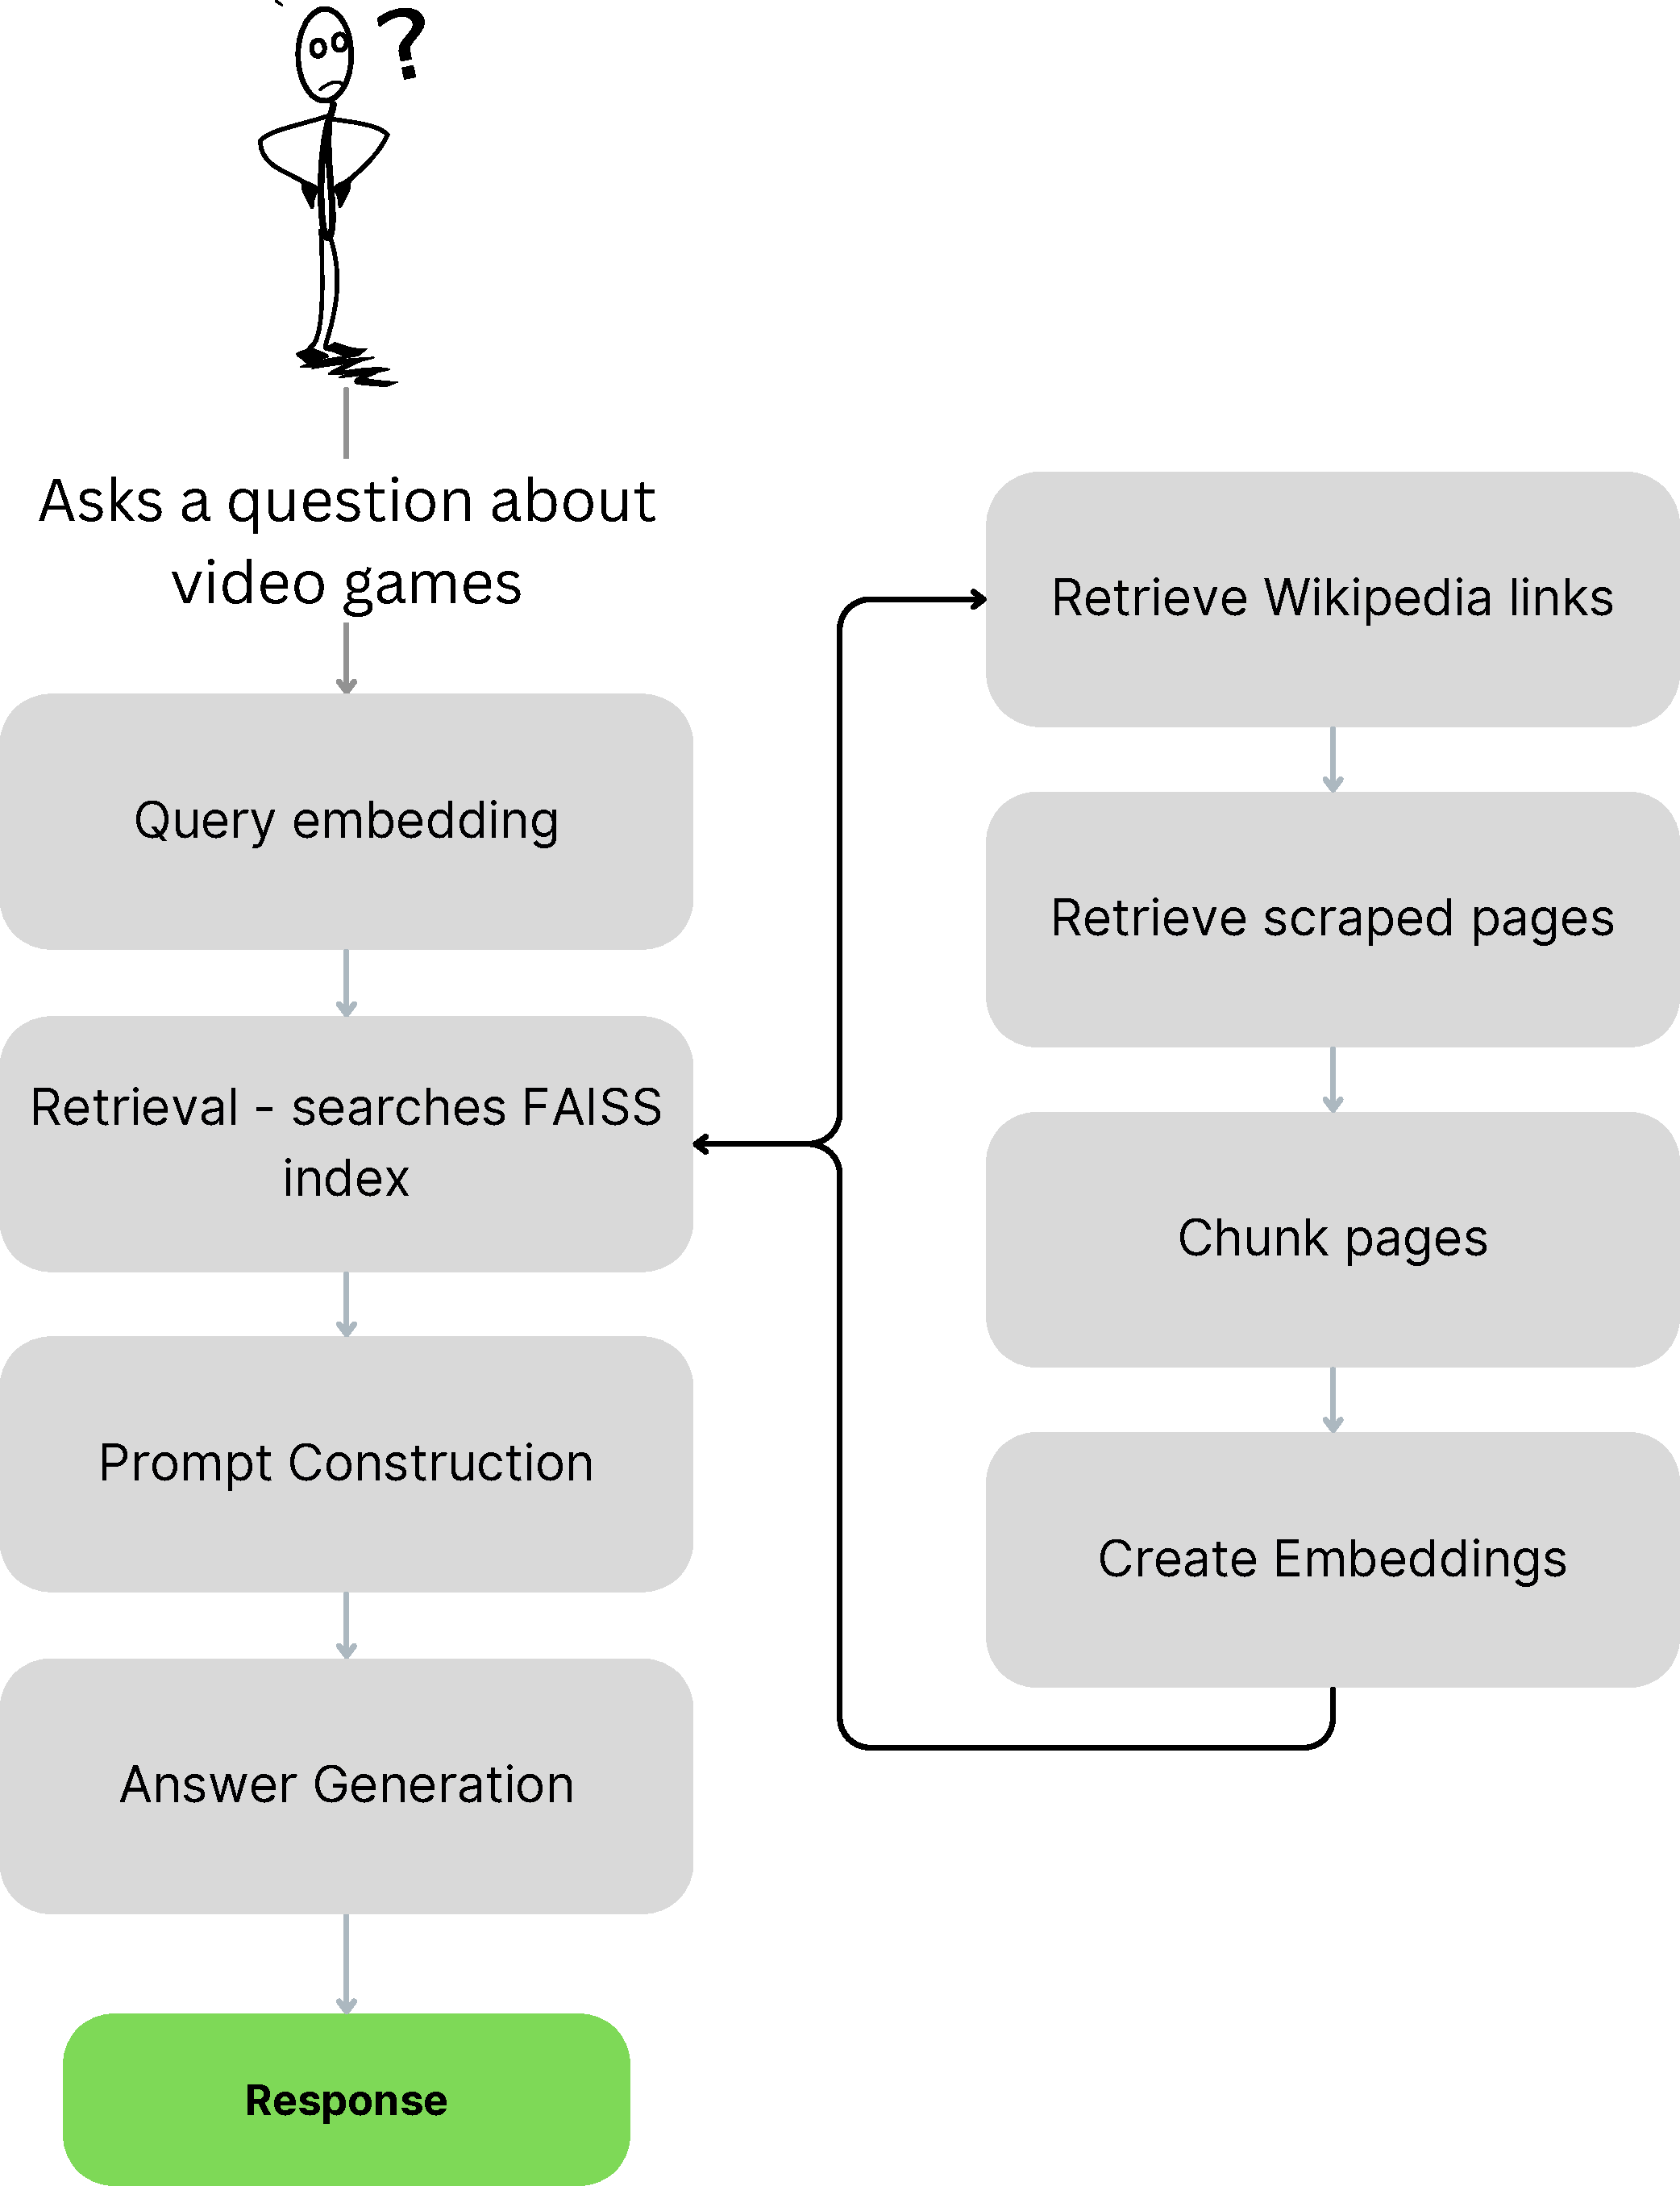
\includegraphics[width=0.7\linewidth]{rag-pipeline.pdf}
    \caption{Baseline RAG pipeline.}
    \label{fig:rag-pipeline}
\end{figure}

Additionally, for testing this live retrieval setup, we reused the original set of 10 factual questions developed during the initial implementation phase. To further evaluate performance and robustness, we also authored an additional 30 questions focused on upcoming video games, maintaining thematic consistency with the original benchmark while expanding the test coverage.

The complete architecture of this dynamic RAG system is illustrated in Figure~\ref{fig:rag-pipeline}. This live-retrieval pipeline addresses many of the limitations of the earlier version: it supports up-to-date queries, avoids pre-embedding the full corpus, and eliminates the need to maintain a large, static index. It also reduces development friction when evaluating performance on current or time-sensitive topics.

\section*{Results}

In this section, we present a series of experiments evaluating the performance of our retrieval-augmented generation (RAG) system. We analyze the impact of retrieval, retrieval configuration parameters, and underlying language models using quantitative metrics across multiple dimensions.

\subsection*{Impact of Retrieval on Model Performance}
We first aimed to verify whether our retrieval mechanism improves the performance of the base language model. To this end, we evaluated the impact of our improved retrieval-augmented generation (RAG) system using the base model \textit{deepseek-ai/deepseek-llm-7b-chat}. To quantify the effect of retrieval, we compared model performance with and without retrieval using three key metrics: {Correctness}, {Semantic Similarity}, and {Relevance}.

\textit{Correctness} was manually assessed by human annotators, who verified whether the model's response accurately and sufficiently answered the posed question. Here is an example of a correctly answered question:

\begin{tcolorbox}[colback=gray!10!white, colframe=gray!80!black, boxrule=0.8pt, arc=3pt, left=3pt, right=3pt, top=3pt, bottom=3pt]
\textbf{Question:} When is GTA VI coming out?

\vspace{6pt}
\textbf{Answer:} GTA VI is coming out on May 26, 2026.
\end{tcolorbox}

\textit{Semantic Similarity} was computed by embedding both the reference (ground truth) and the model-generated answer using a sentence embedding model, and then measuring the cosine similarity between the two embeddings. The ground truth answers were generated using the GPT-4o model \cite{openai}, which answered the questions with access to web search to ensure accurate and up-to-date responses. This metric captures how close the generated answer is in meaning to the reference answer, even if the wording is different. 

\textit{Relevance} was measured by prompting GPT-4o with the question and the model's answer, and asking it to rate how well the answer addressed the question on a scale from 0 to 1, where 0 indicates completely irrelevant and 1 indicates a fully relevant and appropriate response.

The retrieval setup involved a chunk size of 512 tokens, querying content from two pages per prompt, and selecting the top 5 most relevant chunks.

\begin{table}[ht]
\caption{Comparison of RAG performance with and without retrieval using targeted metrics.}
\centering
\begin{tabular}{lcc}
\toprule
\textbf{Metric} & \textbf{Without Retrieval} & \textbf{With Retrieval} \\
\midrule
Correctness & 0.18 & 0.80 \\
Semantic Similarity & 0.23 & 0.73 \\
Relevance & 0.54 & 0.83 \\
\bottomrule
\end{tabular}
\label{tab:rag_core_metrics}
\end{table}

As shown in Table~\ref{tab:rag_core_metrics}, the inclusion of retrieval results in a substantial performance boost across all evaluation metrics.

\subsection*{Effect of Number of Retrieved Pages}
Next, we investigated the effect of varying the number of retrieved pages on the RAG system's performance. We used the same base model with a chunk size of 512 tokens and selected the top 5 most relevant chunks for each query. Table~\ref{tab:rag_pages_key_metrics} summarizes the results across different retrieval sizes: 1, 2, 5, and 10 pages. 

\begin{table}[ht]
\caption{Comparison of RAG performance for different numbers of retrieved pages using key evaluation metrics.}
\centering
\begin{tabular}{lcccc}
\toprule
\textbf{Metric} & \textbf{1} & \textbf{2} & \textbf{5} & \textbf{10} \\
\midrule
Correctness & 0.73 & 0.80 & 0.88 & 0.73 \\
Semantic Similarity & 0.70 & 0.73 & 0.72 & 0.70 \\
Relevance & 0.87 & 0.83 & 0.87 & 0.85 \\
\bottomrule
\end{tabular}
\label{tab:rag_pages_key_metrics}
\end{table}

As shown in the table, retrieving only 1 page often provided insufficient information, resulting in lower correctness and semantic similarity. Increasing to 2 pages significantly improved these metrics by providing more relevant content. At 5 pages, correctness peaked, indicating an optimal balance between useful information and noise. However, retrieving 10 pages led to a decline in performance, likely due to information overload causing less focused answers. Despite stable relevance scores, semantic similarity and correctness dropped compared to 5 pages. These findings emphasize the need to carefully select the retrieval size to enhance model performance without overwhelming it.

\subsection*{Effect of Chunk Size on Performance}
We analyzed the impact of different chunking sizes on RAG performance.  As in previous experiments, we used the same model, retrieving the top 5 chunks from a total of 2 pages per query.

\begin{table}[ht]
\caption{Comparison of RAG performance for different chunk sizes using key evaluation metrics.}
\centering
\begin{tabular}{lcccc}
\toprule
\textbf{Metric} & \textbf{128} & \textbf{256} & \textbf{512} & \textbf{1024} \\
\midrule
Correctness & 0.78 & 0.78 & 0.80 & 0.88 \\
Semantic Similarity & 0.74 & 0.69 & 0.73 & 0.71 \\
Relevance & 0.87 & 0.84 & 0.83 & 0.87 \\
\bottomrule
\end{tabular}
\label{tab:rag_chunk_key_metrics}
\end{table}

As shown in Table~\ref{tab:rag_chunk_key_metrics}, larger chunk sizes generally led to slightly better correctness scores. This suggests that larger chunks may provide more complete context within a single retrieval unit, helping the model generate more accurate answers. However, the improvement comes with potential trade-offs: larger chunks may include more irrelevant information, which can dilute the focus of retrieval and slightly reduce semantic similarity, as seen with the 1024 setting. Despite this, relevance remained relatively stable across all chunk sizes, indicating the model's robustness to chunking variation.

\subsection*{Impact of Number of Retrieved Chunks}
Then we examined how the number of retrieved chunks affects RAG performance.

\begin{table}[ht]
\caption{Comparison of RAG performance for different numbers of retrieved chunks using key evaluation metrics.}
\centering
\begin{tabular}{lcccc}
\toprule
\textbf{Metric} & \textbf{1} & \textbf{3} & \textbf{5} & \textbf{10} \\
\midrule
Correctness & 0.88 & 0.93 & 0.80 & 0.93 \\
Semantic Similarity & 0.72 & 0.70 & 0.73 & 0.72 \\
Relevance & 0.86 & 0.86 & 0.83 & 0.88 \\
\bottomrule
\end{tabular}
\label{tab:rag_chunk_retrieval_metrics}
\end{table}

In Table~\ref{tab:rag_chunk_retrieval_metrics}, we present results for retrieving 1, 3, 5, and 10 chunks. The results show only minor variation and no clear upward or downward trend. We initially expected that retrieving more chunks would either improve performance—by providing more relevant information—or deteriorate it—by overwhelming the model with noise. However, this was not observed. The inconsistency likely stems from the fact that, in many cases, the necessary information was already present in the first few chunks, making the total number of retrieved chunks less impactful. This suggests that the effectiveness of chunk retrieval depends more on the quality and relevance of the top-ranked chunks than on the quantity retrieved.

\subsection*{Comparison Across Language Models}

Lastly, we evaluated the performance of different LLMs under the same conditions to understand how model size and architecture affect output quality. The models tested were: \textbf{A} = \textit{deepseek-ai/deepseek-llm-7b-chat}, \textbf{B} = \textit{DeepSeek-R1-Distill-Qwen-14B}, and \textbf{C} = \textit{sarvamai/sarvam-m-26B} \cite{sarvam2025sarvam}. All models received the same prompts, and we aimed to keep the retrieval parameters consistent across runs.

\begin{table}[ht]
\caption{Comparison of performance metrics across different language models.}
\centering
\begin{tabular}{lccc}
\toprule
\textbf{Metric} & \textbf{A} & \textbf{B} & \textbf{C} \\
\midrule
Correctness & 0.80 & 0.75 & 0.70 \\
Semantic Similarity & 0.73 & 0.66 & 0.50 \\
Relevance & 0.83 & 0.80 & 0.68 \\
\bottomrule
\end{tabular}
\label{tab:model_comparison}
\end{table}

As shown in Table~\ref{tab:model_comparison}, it is surprising that the largest model, \textit{Sarvam-M-26B}, performed worst across all metrics. We initially expected it to outperform smaller models due to its size and potential for richer understanding. However, the decline in semantic similarity and relevance suggests that the model may not have been optimized for our prompting format or task setup. Notably, \textit{Sarvam-M-26B} may require specialized prompting or fine-tuning, which we did not apply—this could explain its underperformance. Additionally, we suspect retrieval played a role; if relevant content wasn’t effectively surfaced, the model could not leverage its full potential. Interestingly, the smaller \textit{DeepSeek-7B} model performed best overall, highlighting how alignment and compatibility with the retrieval setup can be just as important as raw model size.

\section*{Discussion}

This work presents a modular Retrieval-Augmented Generation (RAG) pipeline using live Wikipedia data to answer factual queries. Through controlled experiments, we analyzed the effects of retrieval, chunk size, number of pages and chunks retrieved, and language model selection.

Our findings show that our retrieval has a strong positive impact on answer quality. Including relevant context significantly improved the model’s performance across all evaluation criteria. The best results were achieved when retrieving a moderate number of pages and using medium-to-large chunk sizes, which offered a good balance between context depth and relevance. Interestingly, increasing the number of retrieved chunks didn’t consistently improve performance, suggesting that the most relevant information is often contained in the top-ranked results. Surprisingly, a smaller language model outperformed larger ones, emphasizing that compatibility with the retrieval setup and prompt format can matter more than model size alone.

A key limitation lies in query formulation. Since user questions are passed to the retriever without preprocessing, poorly phrased or misaligned queries can lead to irrelevant or incomplete retrieval. This directly limits overall performance.

Future work should explore query enhancement methods—such as query expansion, paraphrasing, or reformulation via auxiliary LLMs—to better align search inputs with Wikipedia content. Improving this step would enhance retrieval quality and allow more powerful models to perform closer to their potential, making the system more robust across diverse queries.


%----------------------------------------------------------------------------------------
%	REFERENCE LIST
%----------------------------------------------------------------------------------------
\bibliographystyle{unsrt}
\bibliography{report}


\end{document}